\chapter{Introduction}\label{intro}

\section{Introduction}
\subsection{Clustering}
Clustering can be considered as the most important \textit{unsupervised learning} problem;
so, as every other problem of this type, it deals with finding a \textit{structure} in a
collection of given unlabeled datasets. A very common informal definition of clustering could be
``the process of organizing objects into groups whose members are similar in some features of the given dataset".
A \textit{cluster} is therefore a collection of objects which are ``similar" between them and are
``dissimilar" to the objects belonging to other clusters.

We can show this with a simple graphical example:

\begin{figure}[h]
  \centering
  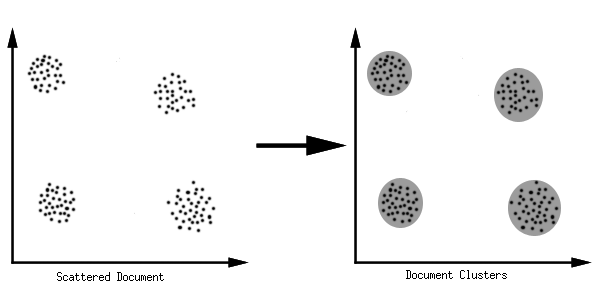
\includegraphics[width=0.9\textwidth]{figures/clustering}
  \caption{Clustering Process}
  \label{fig:clustering}
\end{figure}

In Figure \ref{fig:clustering} we can easily identify the 4 clusters into which the data can be divided; the similarity
criterion is \textit{distance}: two or more objects belong to the same cluster if they are ``close" according to a
given distance (in this case geometrical distance). This is called \textit{distance-based clustering}.
Another kind of clustering is \textit{conceptual clustering}: two or more objects belong to the same cluster
if this one defines a concept common to all that objects. In other words, objects are grouped according
to their fit to descriptive concepts, not according to simple similarity measures.

\subsection{Goals}
The main goal of clustering is to determine the intrinsic grouping in a given set of unlabeled data.
But there is no such factors to decide what constitutes a good clustering. It can be shown that there is no
absolute ``best" criterion which would be independent of the final aim of the clustering. Consequently, it is the user
which must supply this criterion, in such a way that the result of the clustering will suit their needs.
For instance, we could be interested in finding representatives for homogeneous groups (data reduction),
in finding ``natural clusters" and describe their unknown properties (``natural" data types),
in finding useful and suitable groupings (``useful" data classes) or in finding unusual data objects (outlier detection).

\subsection{Applications}
Clustering algorithms can be applied in a very wide range of fields. In \textit{Marketing} we can use clustering
to find groups of customers with similar behavior from a large database of customers data containing their properties
and past buying records. In \textit{Biology} we can classify plants and animals by their given feature sets. Book
ordering and sorting can be a good application of clustering in the \textit{Libraries}. \textit{Insurance} companies
use clustering for identifying groups of insurance policy holders with a high average claim cost.
Recently urban developers are using clustering methods for identifying groups
of houses according to their house type, value and geographical location in \textit{city-planning}. To identify
dangerous zones of earthquake we can observe earthquake epicenters by using clustering algorithms on. These days
clustering algorithms are mostly used in \textit{WWW} for document classification;
clustering weblog data to discover groups of similar access patterns.

\subsection{Requirements}
The main requirements that a clustering algorithm should satisfy are:
\begin{itemize}
\item \textbf{Scalability} : We need highly scalable clustering algorithms to deal with large databases.
\item \textbf{Ability to deal with different kinds of attributes} : Algorithms should be capable to be applied on any kind of data such as interval-based (numerical) data, categorical, and binary data.
\item \textbf{Discovery of clusters with attribute shape} : The clustering algorithm should be capable of detecting clusters of arbitrary shape. They should not be bounded to only distance measures that tend to find spherical cluster of small sizes.
\item \textbf{High dimensionality} : The clustering algorithm should not only be able to handle low-dimensional data but also the high dimensional space.
\item \textbf{Ability to deal with noisy data} : Databases contain noisy, missing or erroneous data. Some algorithms are sensitive to such data and may lead to poor quality clusters.
\item \textbf{Interpretability} : The clustering results should be interpretable, comprehensible, and usable.
\end{itemize}

\subsection{Problems}
There are a number of problems with clustering. Among them:
\begin{itemize}
\item Current clustering techniques do not address all the requirements adequately (and concurrently);
\item Dealing with large number of dimensions and large number of data items can be problematic because of time complexity;
\item The effectiveness of the method depends on the definition of “distance” (for distance-based clustering);
\item If an obvious distance measure doesn’t exist we must “define” it, which is not always easy, especially in multi-dimensional spaces;
\item The result of the clustering algorithm (that in many cases can be arbitrary itself) can be interpreted in different ways.
\end{itemize}

\subsection{Classification}
Clustering algorithms may be classified as listed below:
\begin{itemize}
\item \textbf{Hierarchical Clustering} : Hierarchical clustering, is based on the core idea of objects being more
related to nearby objects than to objects farther away. These algorithms connect ``objects" to form ``clusters"
based on their distance. A cluster can be described largely by the maximum distance needed to connect parts of
the cluster. At different distances, different clusters will form, which can be represented using a \textit{dendrogram},
which explains where the common name ``Hierarchical Clustering" comes from: these algorithms do not provide a
single partitioning of the data set, but instead provide an extensive hierarchy of clusters that merge with each
other at certain distances. In a dendrogram, the Y-axis marks the distance at which the clusters merge, while the
objects are placed along the X-axis such that the clusters don't mix.

Connectivity based clustering is a whole family of methods that differ by the way distances are computed.
Apart from the usual choice of \textit{distance functions}, the user also needs to decide on the linkage criterion
(since a cluster consists of multiple objects, there are multiple candidates to compute the distance to) to use.
Popular choices are known as \textit{single-linkage clustering} (the minimum of object distances),
\textit{complete linkage clustering} (the maximum of object distances) or UPGMA (``Unweighted Pair Group Method with
Arithmetic Mean", also known as average linkage clustering). Furthermore, hierarchical clustering can be
agglomerative (starting with single elements and aggregating them into clusters) or divisive
(starting with the complete data set and dividing it into partitions).

These methods will not produce a unique partitioning of the data set, but a hierarchy from which the user still
needs to choose appropriate clusters. They are not very robust towards outliers, which will either show up as
additional clusters or even cause other clusters to merge (known as ``chaining phenomenon", in particular with
single-linkage clustering). In the general case, the complexity is $O(n^{3})$ for agglomerative clustering and
$O(2^{n-1})$ for \textit{divisive clustering}, which makes them too slow for large data sets. For some special cases,
optimal efficient methods (of complexity $O(n^{2})$ are known as single-linkage and complete-linkage clustering.
In the \textit{data mining} community these methods are recognized as a theoretical foundation of cluster analysis,
but often considered obsolete. They did however provide inspiration for many later methods such as density based
clustering.


\item \textbf{Centroid-based Clustering} : In centroid-based clustering, clusters are represented by a central vector,
which may not necessarily be a member of the data set. When the number of clusters is fixed to k, k-means clustering
gives a formal definition as an optimization problem: find the k cluster centers and assign the objects to the nearest
cluster center, such that the squared distances from the cluster are minimized.

The optimization problem itself is known to be NP-hard, and thus the common approach is to search only for approximate
solutions. A particularly well known approximative method is Lloyd's algorithm, often actually referred to as
``k-means algorithm". It does however only find a local optimum, and is commonly run multiple times with different
random initializations. Variations of k-means often include such optimizations as choosing the best of multiple runs,
but also restricting the centroids to members of the data set (k-medoids), choosing medians (k-medians clustering),
choosing the initial centers less randomly (k-means++) or allowing a fuzzy cluster assignment (fuzzy c-means).

Most k-means-type algorithms require the number of clusters - k to be specified in advance, which is considered
to be one of the biggest drawbacks of these algorithms. Furthermore, the algorithms prefer clusters of approximately
similar size, as they will always assign an object to the nearest centroid. This often leads to incorrectly cut
borders of clusters (which is not surprising since the algorithm optimizes cluster centers, not cluster borders).

\item \textbf{Distribution-based clustering} : The clustering model most closely related to statistics is based
on distribution models. Clusters can then easily be defined as objects belonging most likely to the same distribution.
A convenient property of this approach is that this closely resembles the way artificial data sets are generated:
by sampling random objects from a distribution.

While the theoretical foundation of these methods is excellent, they suffer from one key problem known as overfitting,
unless constraints are put on the model complexity. A more complex model will usually be able to explain the data better,
which makes choosing the appropriate model complexity inherently difficult.

One prominent method is known as Gaussian mixture models (using the expectation-maximization algorithm). Here,
the data set is usually modelled with a fixed (to avoid overfitting) number of Gaussian distributions that are
initialized randomly and whose parameters are iteratively optimized to better fit the data set. This will converge
to a local optimum, so multiple runs may produce different results. In order to obtain a hard clustering, objects
are often then assigned to the Gaussian distribution they most likely belong to; for soft clusterings, this is not
necessary.

Distribution-based clustering produces complex models for clusters that can capture correlation and dependence
between attributes. However, these algorithms put an extra burden on the user: for many real data sets, there may
be no concisely defined mathematical model (e.g. assuming Gaussian distributions is a rather strong assumption
on the data).

\item \textbf{Density-based Clustering} : In density-based clustering, clusters are defined as areas of higher density
than the remainder of the data set. Objects in these sparse areas - that are required to separate clusters - are usually
considered to be noise and border points.

The most popular density based clustering method is DBSCAN. In contrast to many newer methods, it features a well-defined
cluster model called ``density-reachability". Similar to linkage based clustering, it is based on connecting points within
certain distance thresholds. However, it only connects points that satisfy a density criterion, in the original variant
defined as a minimum number of other objects within this radius. A cluster consists of all density-connected objects
(which can form a cluster of an arbitrary shape, in contrast to many other methods) plus all objects that are within
these objects' range. Another interesting property of DBSCAN is that its complexity is fairly low - it requires a linear
number of range queries on the database - and that it will discover essentially the same results (it is deterministic
for core and noise points, but not for border points) in each run, therefore there is no need to run it multiple times.
OPTICS is a generalization of DBSCAN that removes the need to choose an appropriate value for the range parameter ${\varepsilon}$,
and produces a hierarchical result related to that of linkage clustering. DeLi-Clu, Density-Link-Clustering combines ideas
from single-linkage clustering and OPTICS, eliminating the ${\varepsilon}$ parameter entirely and offering performance improvements
over OPTICS by using an R-tree index.

The key drawback of DBSCAN and OPTICS is that they expect some kind of density drop to detect cluster borders.
On data sets with, for example, overlapping Gaussian distributions - a common use case in artificial data - the
cluster borders produced by these algorithms will often look arbitrary, because the cluster density decreases
continuously. On a data set consisting of mixtures of Gaussians, these algorithms are nearly always outperformed
by methods such as EM clustering that are able to precisely model this kind of data.

Mean-shift is a clustering approach where each object is moved to the densest area in its vicinity, based on kernel
density estimation. Eventually, objects converge to local maxima of density. Similar to k-means clustering, these
``density attractors" can serve as representatives for the data set, but mean-shift can detect arbitrary-shaped
clusters similar to DBSCAN. Due to the expensive iterative procedure and density estimation, mean-shift is usually
slower than DBSCAN or k-Means. Besides that, the applicability of the mean-shift algorithm to multidimensional data
is hindered by the unsmooth behaviour of the kernel density estimate, which results in over-fragmentation of cluster
tails.
\end{itemize}

\section{Literature Survey}

\subsection{Distance Measure}
An important component of a clustering algorithm is the distance measure between data points. If the components of the data instance vectors are all in the same physical units then it is possible that the simple Euclidean distance metric is sufficient to successfully group similar data instances. However, even in this case the Euclidean distance can sometimes be misleading. Figure shown below illustrates this with an example of the width and height measurements of an object. Despite both measurements being taken in the same physical units, an informed decision has to be made as to the relative scaling. As the figure shows, different scalings can lead to different clusterings.
Notice however that this is not only a graphic issue: the problem arises from the mathematical formula used to combine the distances between the single components of the data feature vectors into a unique distance measure that can be used for clustering purposes: different formulas leads to different clusterings.
Again, domain knowledge must be used to guide the formulation of a suitable distance measure for each particular application.

\section{Research Gap}

\section{Objective}

\section{Thesis Organization}



\section{Cross Referencing}
We have incorporated the \verb@\cref@ or \verb@\Cref@ command from
\texttt{cleveref} package in this system. This will automatically
insert words like Figure, Table etc.\ in your text.

See these examples:
\begin{itemize}
\item \Cref{fig:sample} is a sample figure.
\item \Cref{tab_our} is a table.
\item \Cref{sec:cite} in \Cref{ch:citations} shows some examples of
  citations.
\end{itemize}

\section{How to Write a Section}

This is for writing section.

\section{How to Add Table and Figures}\label{contribution}
You should refer a figure as, ``\Cref{fig:sample} is a sample
figure''.




Then we applied same test cases to our modified algorithm i.e.\ the
heuristic algorithm with our new operation \textit{Block Reversal}. The
performance is shown in \Cref{tab_our}.


\begin{table}[!tb]
  \begin{center}
    \caption{Performance table of \emph{Block reversal} in a heuristic algorithm}
    \label{tab_our}

    \begin{tabular}{|l|r|r|r|r|r|r|r|r|r|r|r|r|r|}
      \hline
      $\alpha$     & $\alpha n$ & \multicolumn{11}{c|}{Test Cases} & \multicolumn{1}{c|}{Average \# of}                                     \\
      \cline{3-13} &            & 1                                & 2  & 3  & 4  & 5  & 6  & 7  & 8  & 9  & 10 & 11 & calculated operation \\
      \hline
      0.1        & 2          & 2                                & 2	& 2  & 2  & 2  & 2  & 2  & 2  &	2  & 2	& 2  & 2                    \\
      0.2        & 4          & 4                                & 4	& 5  & 2  & 4  & 4  & 4  & 4  &	2  & 4	& 4  & 3.73                 \\
      0.3        & 6          & 5                                & 6	& 6  & 6  & 6  & 7  & 6  & 5  &	6  & 6	& 6  & 5.91                 \\
      0.4        & 8          & 7                                & 8	& 5  & 6  & 7  & 6  & 6  & 7  &	8  & 8	& 7  & 6.82                 \\
      0.5        & 10         & 9                                & 10	& 6  & 12 & 10 & 8  & 10 & 10 &	7  & 7	& 10 & 9                    \\
      0.6        & 12         & 9                                & 12	& 16 & 10 & 12 & 12 & 9  & 11 &	12 & 9	& 12 & 11.27                \\
      0.7        & 14         & 13                               & 7	& 18 & 15 & 14 & 8  & 13 & 11 &	13 & 13	& 14 & 12.64                \\
      0.8        & 16         & 10                               & 17	& 14 & 16 & 13 & 16 & 13 & 11 &	13 & 17	& 13 & 13.91                \\
      0.9        & 18         & 14                               & 16	& 15 & 12 & 15 & 11 & 15 & 11 &	15 & 12	& 12 & 13.45                \\
      1          & 20         & 18                               & 11	& 13 & 11 & 13 & 15 & 17 & 17 &	13 & 18	& 12 & 14.36                \\
      \hline
    \end{tabular}
  \end{center}
\end{table}


These are some dummy text used as page fillers only.

Lorem ipsum dolor sit amet, consectetur adipiscing elit. Cras et
ultricies massa. Nulla a sapien lobortis, dignissim nibh in, aliquet
mauris. Integer at dictum metus. Quisque in tortor congue ipsum
ultricies tristique. Maecenas ut tortor dapibus, sagittis enim at,
tincidunt massa. Ut sollicitudin sagittis ipsum, ac tincidunt quam
gravida ac. Nullam quis faucibus purus. Aliquam vel pretium
turpis. Aliquam a quam non ex interdum sagittis id vitae quam. Nullam
sodales ligula malesuada maximus consequat. Proin a justo eget lacus
vulputate maximus luctus vitae enim. Aliquam libero turpis, pharetra a
tincidunt ac, pulvinar sit amet urna. Pellentesque eget rutrum diam,
in faucibus sapien. Aenean sit amet est felis. Aliquam dolor eros,
porttitor quis volutpat eget, posuere a ligula. Proin id velit ac
lorem finibus pellentesque.

Maecenas vitae interdum mi. Aenean commodo nisl massa, at pharetra
libero cursus vitae. In hac habitasse platea dictumst. Suspendisse
iaculis euismod dui, et cursus diam. Nullam euismod, est ut dapibus
condimentum, lorem eros suscipit risus, sit amet hendrerit justo
tortor nec lorem. Morbi et mi eget erat bibendum porta. Ut tristique
ultricies commodo. Nullam iaculis ligula sed lacinia ornare.

Sed ultricies cursus nisi at vestibulum. Aenean laoreet viverra
efficitur. Ut eget sapien lorem. Mauris malesuada, augue in pulvinar
consectetur, ex tortor tristique ligula, sit amet faucibus metus
lectus interdum nisl. Nam eget turpis vitae ligula pulvinar bibendum a
ut ipsum. Mauris fringilla lacinia malesuada. Fusce id orci
velit. Donec tristique rhoncus urna, a hendrerit arcu vehicula
imperdiet. Integer tristique erat at gravida condimentum. Sed ornare
cursus quam, eget tincidunt enim bibendum sed. Aliquam elementum
ligula scelerisque leo sagittis, quis convallis elit dictum. Donec sit
amet orci aliquam, ultricies sapien nec, gravida nisi. Etiam et
pulvinar diam, et pellentesque arcu. Nulla interdum metus sed aliquet
consequat.

Proin in mi id nulla interdum aliquet ac quis arcu. Duis blandit
sapien commodo turpis hendrerit pharetra. Phasellus sit amet justo
orci. Proin mattis nisl dictum viverra fringilla. Interdum et
malesuada fames ac ante ipsum primis in faucibus. Curabitur facilisis
euismod augue vestibulum tincidunt. Nullam nulla quam, volutpat vitae
efficitur eget, porta sit amet nunc. Phasellus pharetra est eget urna
ornare volutpat. Aenean ultrices, libero eget porttitor fringilla,
purus tortor accumsan neque, sit amet viverra felis tortor eget
justo. Nunc id metus a purus tempus euismod condimentum non lacus. Nam
vitae diam aliquam, facilisis diam quis, pharetra nunc. Nulla eget
vestibulum tellus, ut cursus tellus. Vestibulum euismod pellentesque
sodales.

Maecenas at mi interdum, faucibus lorem sed, hendrerit nisi. In vitae
augue consequat diam commodo porta sit amet eu purus. Mauris mattis
condimentum feugiat. Nulla commodo molestie risus vitae maximus. Proin
hendrerit neque malesuada urna laoreet convallis. Etiam a diam
pulvinar, auctor sem ac, hendrerit risus. Ut urna urna, venenatis ac
tellus non, scelerisque tristique ligula. Vestibulum sollicitudin vel
leo malesuada accumsan. Donec sit amet erat diam. Vestibulum ante
ipsum primis in faucibus orci luctus et ultrices posuere cubilia
Curae; Vivamus odio dui, scelerisque et lorem egestas, posuere
ullamcorper nunc. Integer varius nunc nec velit tincidunt
commodo. Mauris rhoncus ultrices sapien non suscipit.


End of dummy text.


\endinput
